%%
%% This is file `sample-authordraft.tex',
%% generated with the docstrip utility.
%%
%% The original source files were:
%%
%% samples.dtx  (with options: `authordraft')
%% 
%% IMPORTANT NOTICE:
%% 
%% For the copyright see the source file.
%% 
%% Any modified versions of this file must be renamed
%% with new filenames distinct from sample-authordraft.tex.
%% 
%% For distribution of the original source see the terms
%% for copying and modification in the file samples.dtx.
%% 
%% This generated file may be distributed as long as the
%% original source files, as listed above, are part of the
%% same distribution. (The sources need not necessarily be
%% in the same archive or directory.)
%%
%% The first command in your LaTeX source must be the \documentclass command.
\documentclass[sigconf,authordraft]{acmart}
\settopmatter{printacmref=false} % Removes citation information below abstract
\renewcommand\footnotetextcopyrightpermission[1]{} % removes footnote with conference information in first column
\pagestyle{plain} % removes running headers

\definecolor{pink}{rgb}{0.9,0,0.9}
 
\newcommand{\hilight}[1]{\colorbox{yellow}{#1}}
\newcommand{\jg}[1]{\textbf{\textcolor{pink}{#1}}}


\usepackage{menukeys}
%%
%% \BibTeX command to typeset BibTeX logo in the docs
\AtBeginDocument{%
  \providecommand\BibTeX{{%
    \normalfont B\kern-0.5em{\scshape i\kern-0.25em b}\kern-0.8em\TeX}}}

%% Rights management information.  This information is sent to you
%% when you complete the rights form.  These commands have SAMPLE
%% values in them; it is your responsibility as an author to replace
%% the commands and values with those provided to you when you
%% complete the rights form.
\setcopyright{acmcopyright}
\copyrightyear{2018}
\acmYear{2018}
\acmDOI{10.1145/1122445.1122456}

%% These commands are for a PROCEEDINGS abstract or paper.
% \acmConference[Woodstock '18]{Woodstock '18: ACM Symposium on Neural
%   Gaze Detection}{June 03--05, 2018}{Woodstock, NY}
% \acmBooktitle{Woodstock '18: ACM Symposium on Neural Gaze Detection,
%   June 03--05, 2018, Woodstock, NY}
% \acmPrice{15.00}
% \acmISBN{978-1-4503-9999-9/18/06}


%%
%% Submission ID.
%% Use this when submitting an article to a sponsored event. You'll
%% receive a unique submission ID from the organizers
%% of the event, and this ID should be used as the parameter to this command.
%%\acmSubmissionID{123-A56-BU3}

%%
%% The majority of ACM publications use numbered citations and
%% references.  The command \citestyle{authoryear} switches to the
%% "author year" style.
%%
%% If you are preparing content for an event
%% sponsored by ACM SIGGRAPH, you must use the "author year" style of
%% citations and references.
%% Uncommenting
%% the next command will enable that style.
%%\citestyle{acmauthoryear}

%%
%% end of the preamble, start of the body of the document source.
\begin{document}

%%
%% The "title" command has an optional parameter,
%% allowing the author to define a "short title" to be used in page headers.
\title{Generating Trace Links from Code to Documentation}

%%
%% The "author" command and its associated commands are used to define
%% the authors and their affiliations.
%% Of note is the shared affiliation of the first two authors, and the
%% "authornote" and "authornotemark" commands
%% used to denote shared contribution to the research.
\author{Breandan Considine}
\email{breandan.considine@mail.mcgill.ca}
\affiliation{%
  \institution{McGill University}
}

\author{Jin L.C. Guo}
\email{jguo@cs.mcgill.ca}
\affiliation{%
  \institution{McGill University}
}

%%
%% By default, the full list of authors will be used in the page
%% headers. Often, this list is too long, and will overlap
%% other information printed in the page headers. This command allows
%% the author to define a more concise list
%% of authors' names for this purpose.

%%
%% The abstract is a short summary of the work to be presented in the
%% article.
\begin{abstract}
When writing software, developers must often switch contexts to navigate between source code, search results and documentation. In practice, writing a query and combing through the search results requires a nontrivial amount of manual effort. In our work, we collect a dataset of embedded links and their lexical context, then learn to rank a set of documents containing the link text, based on their contextual relevance. We compare our relevance-based ranking against a frequency-based ranking using a standard set of information retrieval benchmarks. Finally, we demonstrate a selection-based search assistant to facilitate efficient document retrieval by annotating screenshots containing code-related text with trace links to relevant documentation. In addition to the link dataset itself, we provide two code artifacts for the purposes of experimental reproducibility and artifact evaluation:

\begin{itemize}
    \item TraceLink (\href{https://github.com/breandan/tracelink}{https://github.com/breandan/tracelink})
    \item TraceJump (\href{https://github.com/breandan/tracejump}{https://github.com/breandan/tracejump})
\end{itemize}
\end{abstract}

%%
%% The code below is generated by the tool at http://dl.acm.org/ccs.cfm.
%% Please copy and paste the code instead of the example below.
%%


%%
%% Keywords. The author(s) should pick words that accurately describe
%% the work being presented. Separate the keywords with commas.
\keywords{document retrieval, selection-based search, semantic search, content recommendation, software documentation, learning to rank}

%% A "teaser" image appears between the author and affiliation
%% information and the body of the document, and typically spans the
%% page.
% \begin{teaserfigure}
%   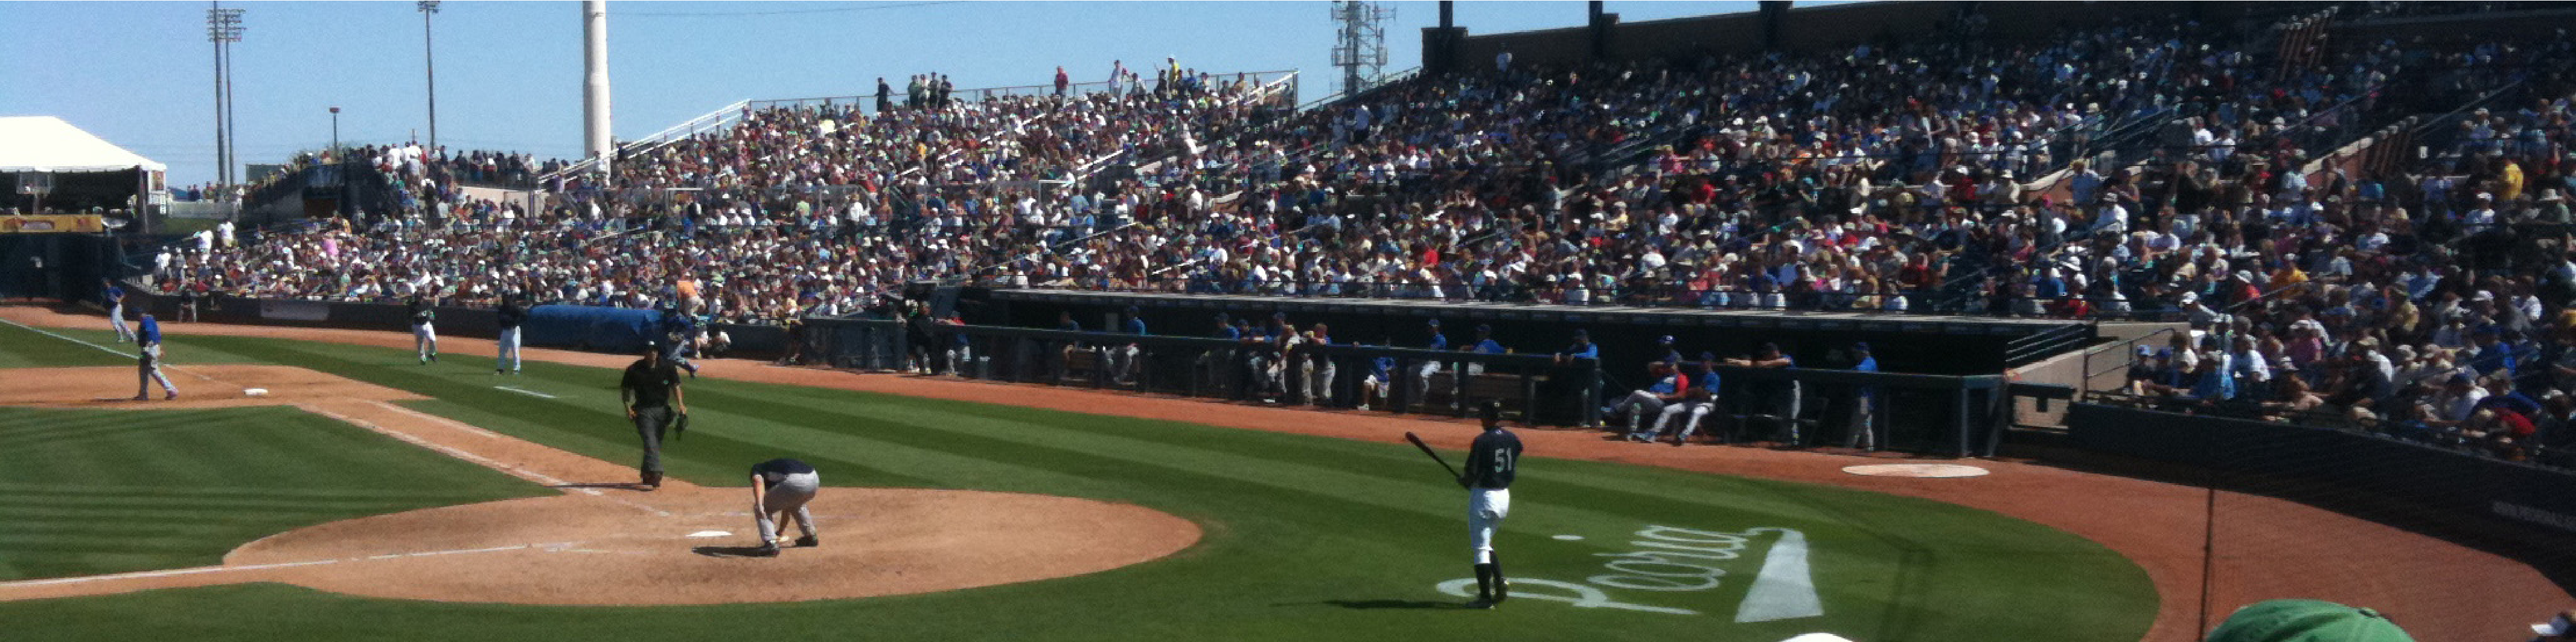
\includegraphics[width=\textwidth]{sampleteaser}
%   \caption{Seattle Mariners at Spring Training, 2010.}
%   \Description{Enjoying the baseball game from the third-base
%   seats. Ichiro Suzuki preparing to bat.}
%   \label{fig:teaser}
% \end{teaserfigure}

%%
%% This command processes the author and affiliation and title
%% information and builds the first part of the formatted document.
\maketitle

\section{Introduction}
\jg{\cite{meng2019developers} to motivate our work "Enable efficient access to relevant content".}
Documentation is an indispensable resource for software developers learning to use a new language, framework or library. Developer documentation is often published in the form of web pages, and later indexed by a search engine. Consider the typical workflow of a software developer seeking information about an unfamiliar API: to effectively locate relevant documentation, developers must first copy a specific fragment of text (e.g. a function name, error message, or identifier) from their development environment into a search engine, alongside some contextual information. This query must be descriptive enough to retrieve relevant documents with high probability, whilst omitting extraneous information (e.g. user defined paths or tokens) unlikely to occur outside the scope of the developer's personal environment or project. The construction of search queries to rapidly locate relevant documentation is a skill which some have colloquially termed "Google-fu". While power users may prefer lexical search (e.g. to retrieve a known document), lexical search can sometimes impede knowledge discovery by requiring developers to articulate the context of a given query, which is often hard to describe succinctly or in the appropriate jargon. Our work seeks to facilitate knowledge discovery by enriching lexical queries with contextual information extracted from the development environment and by prioritizing contextually relevant documentation sources among the search results.

Once the developer has constructed a search query, she may need to check several apparently plausible documents to locate the desired information. After opening a given search result, the desired content is often buried in a long document. To locate the desired information, the user must then construct a secondary search (e.g. via \keys{\ctrl} / \keys{\cmd + F}) to find a specific keyword or phrase, then traverse a list of matches (e.g. via \keys{\return} / \keys{\shift + \return}), visually scanning the surroundings for relevant information. Lexical occurrences from the list could be sorted based on contextually relevance, instead of the sequential order which they appear in most web browsers.

Prior work in information retrieval for software development has investigated recommending documentation \citep{robillard2015recommending} and Stack Overflow content \citep{treude2016augmenting} to developers. Our work roughly falls in the same category as Robillard, Treude, et al. Unlike their approach, we do not require manual content curation and support a broad range of languages and documentation types. \citet{rahman2014towards} explored recommending documentation using lexical similarity, but focuses on a single IDE. More broadly, \citet{el2001linking, dalton2013neighborhood, dalton2014entity} explore entity linking using contextual information in the context of online knowledge bases, but use an outdated bag-of-words (BOW) or n-gram model. Like Dalton et al, our approach prioritizes documents based on semantic or contextual relevance to the query context, but using a sequence embedding. While we focus our attention on linking developer documents in source code, our model is capable of linking entities in any desktop environment or screenshot containing documented code entities.

The rest of this paper is organized as follows. First, we present a novel preprocessing pipeline for extracting links from a corpus of developer documents (or more broadly, any web-based HTML document containing a mixture of source code and natural language). We then describe how to train a language model for ranking a set of lexical search results based on their contextual relevance. We evaluate our ranking function across a standard set of information retrieval benchmarks, such as mean average precision (MAP) and mean reciprocal rank (MRR). We propose a selection-based search assistant for trace link annotation in arbitrary screenshots. Finally, we share a few remarks on the results obtained and potential threats to validity our solution might pose.

\section{Methods}

\subsection{Preprocessing}\label{subsec:preprocessing}

To construct our dataset, we use the \href{https://zealusercontributions.herokuapp.com/}{Zeal User Contributed docsets}, a set of archives containing web-based documentation for many common software libraries, scraped from their official documentation sites. From each document in every docset, we extract a set of links and their surrounding text, i.e. \textit{concordances}. More specifically, each link consists of five distinct features:

\begin{enumerate}
    \item the source document, i.e. uniform resource identifier (URI)
    \item the target document, i.e. uniform resource identifier (URI)
    % \item the subsection identifier (if defined), i.e. the URI fragment
    \item the anchor text, i.e. a single keyword or keyphrase (query)
    % \item the link concordance, i.e. keyword-in-context (KWIC)
    % \item the target document title or subsection heading (if defined)
    % \item the source document title or subsection heading (if defined)
\end{enumerate}

We then search the entire corpus for the anchor text using either direct-hit or fuzzy matching criteria, and return (4) up to 20 candidate documents mentioning the anchor text most frequently, alongside their title and URI. Finally, we apply a form of query expansion~\citep{efthimiadis1996query} to retrieve (5) every concordance of the anchor text in the target document (see Fig.~\ref{fig:concordances}) and the corresponding concordances for each candidate document.~\footnote{See: \href{https://gist.github.com/breandan/226bf08bbd5b394a5d2f2a80d383f726}{https://gist.github.com/breandan/226bf08bbd5b394a5d2f2a80d383f726}} During this process, the document text is stored in an inverted index for full-text search (i.e. including terms which may appear outside links in the dataset).

\begin{figure}
    \centering
    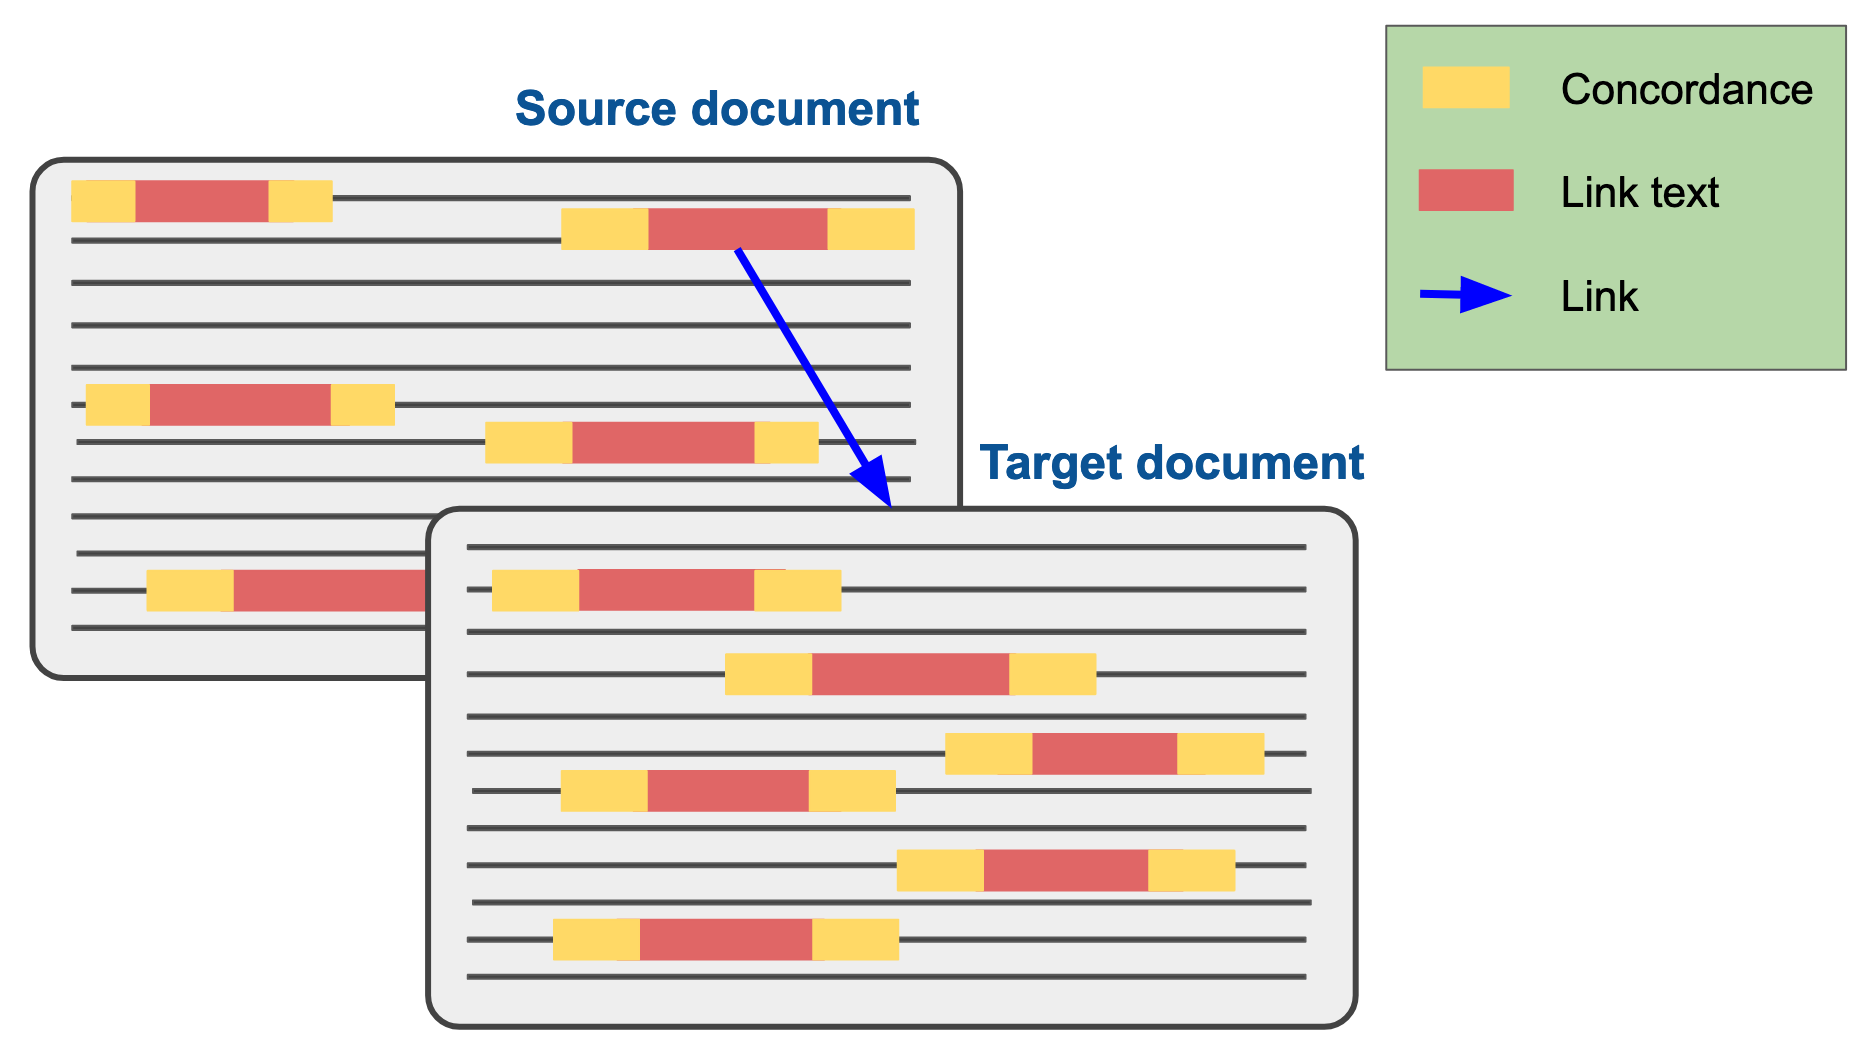
\includegraphics[width=0.4\textwidth,keepaspectratio]{concordance.png}
    \caption{For every link's anchor text, concordances from both the source and target documents are collected.}
    \label{fig:concordances}
\end{figure}

Some links are unrelated to the surrounding concordance. For example, a link may occur inside a table of contents, HTML menu, or boilerplate section. It is further possible, though unlikely, for the anchor text itself to be absent from the target document. To reduce the frequency of atypical links in our dataset, we require all links extracted must conform to the following criteria:

\begin{enumerate}
\item Every URI must point to a valid document in the same docset
\item Source and target URIs must not refer to the same document
\item Candidates must contain both source and target documents
\item Anchor text must occur 2+ times in both source and target
\item No link feature may contain any non-ASCII characters
\item Anchor text must fall between 5 and 50 characters in length
\item Anchor text must not contain any whitespace characters
\end{enumerate}

Many of the links collected have natural language concordances which are unlikely to occur within the context of a development environment. Occasionally, links simply do not contain any code tokens whatsoever. We have tried various heuristics to reduce the proportion of such links in our dataset, such as including only links nearby \texttt{<code>} blocks, using orthographic features like naming convention (e.g. camel case, snake case, kebab case) and code-like punctuation (e.g. brackets, colons and other delimiters), but such heuristics are prone to reduce the lexical diversity which legitimate code-like text is likely to exhibit. However inspection of the dataset reveals most links have code-like tokens either in the anchor text or surrounding concordance, as inbound links on API documentation sites often refer to code-related entities. We discuss the implications of the domain mismatch problem further in Section~\ref{subsec:threats}.

It is possible, although unlikely, for multiple links with the same anchor text and different target URIs to appear within a single document, in which case only the first link occurrence is recorded. Furthermore, only links with unique features are recorded. For example, if two links with identical concordances are found anywhere in the corpus, only the first occurrence is recorded to prevent imbalance arising from boilerplate text (e.g. which may occur in a table of contents or unrelated page structure).

Our test set is comprised of a random 10\% of links from the corpus with exactly the same structure, but with the identity of the target document hidden. Our goal at test time is to predict which document from the list of candidates was the original link target.


\section{Results}

As expected, for link prediction on anchor text contained in the training set, we outperform frequency-based ranking using top-5 prediction accuracy (see Fig.~\ref{fig:training_set}), however further training is required for competitive performance on the test set (see Fig.~\ref{fig:test_set}).

\begin{figure}
    \centering
    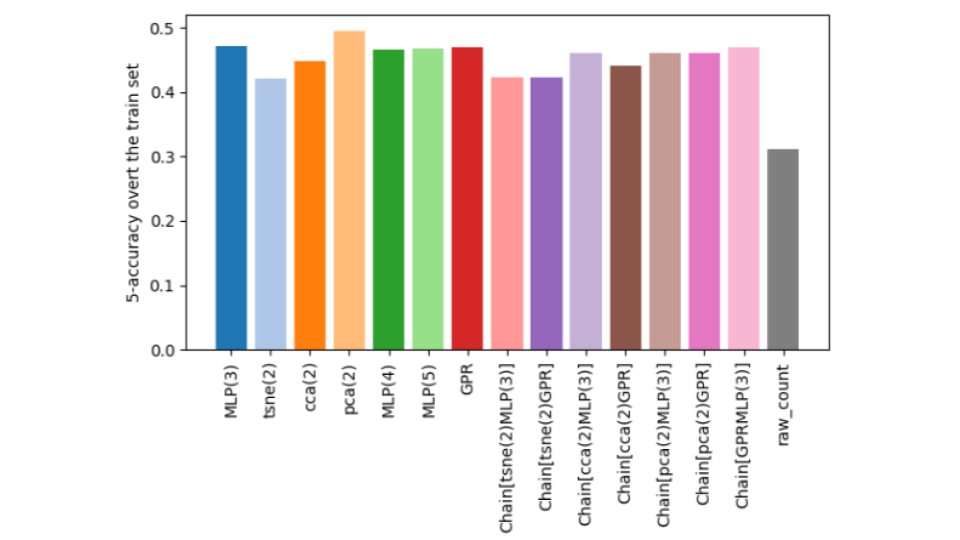
\includegraphics[width=0.4\textwidth,keepaspectratio]{training_set.png}
    \caption{Training set precision using pretrained embedding.}
    \label{fig:training_set}
\end{figure}

\begin{figure}
    \centering
    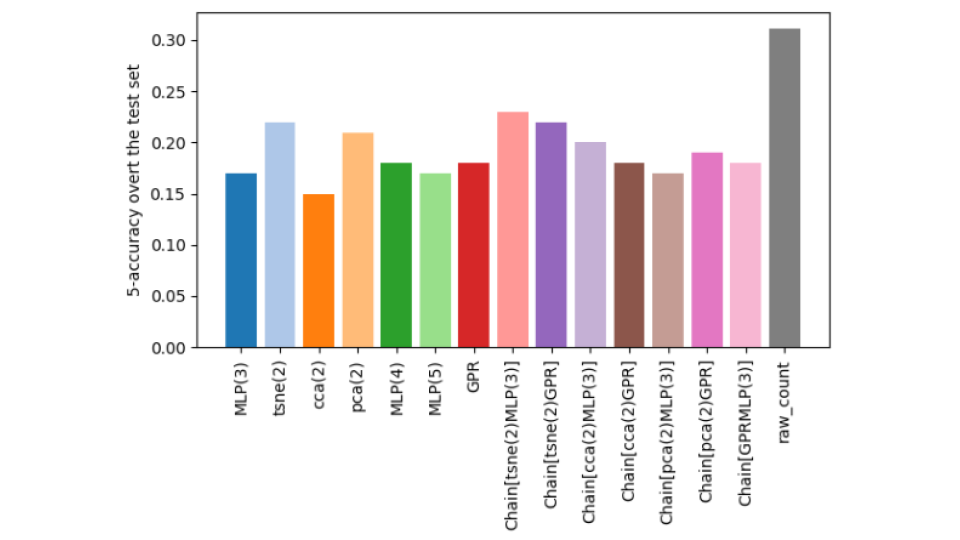
\includegraphics[width=0.4\textwidth,keepaspectratio]{test_set.png}
    \caption{Test set precision using pretrained embedding.}
    \label{fig:test_set}
\end{figure}

\subsection{Trace Link Annotation}

Most trace link annotation tools are based on application-specific workbenches such as DoCIT~\citep{guo2014towards} or embedded as plugins within an integrated development environment such as TraceViz~\citep{marcus2005and}. We present a tool capable of annotating trace links in arbitrary development environments such as terminal emulators, integrated development environments, desktop applications, or even screenshots containing code-related text. Below, we describe the implementation of such a tool, called \textit{TraceJump}.

TraceJump relies on Tesseract~\citep{smith2007overview}, an optical character recognition (OCR) library and JavaFX, a library for building desktop applications. To use the tool, the user first invokes a keyboard command (\keys{\ctrl + \textbackslash} by default), triggering a screen capture. Using Tesseract, we perform OCR on the screenshot and filter each term by a TFIDF threshold. Using JavaFX, we highlight a subset of terms exceeding the threshold over the OCR-segmented text (see Fig.~\ref{fig:tracejump}), which represent expandable trace links. The user can then select a trace link (either directly with their cursor or by typing the adjacent two-letter code), to execute a query over the dataset. Using the inverted index constructed during the preprocessing stage, we retrieve all documents in which the keyword occurs with accompanying concordances. The expanded candidate documents are ranked by their relevance to the screen contents and displayed in KWIC~\citep{luhn1960key} format for document preview, which can be selected to view the corresponding document in a web browser.

\begin{figure}
    \centering
    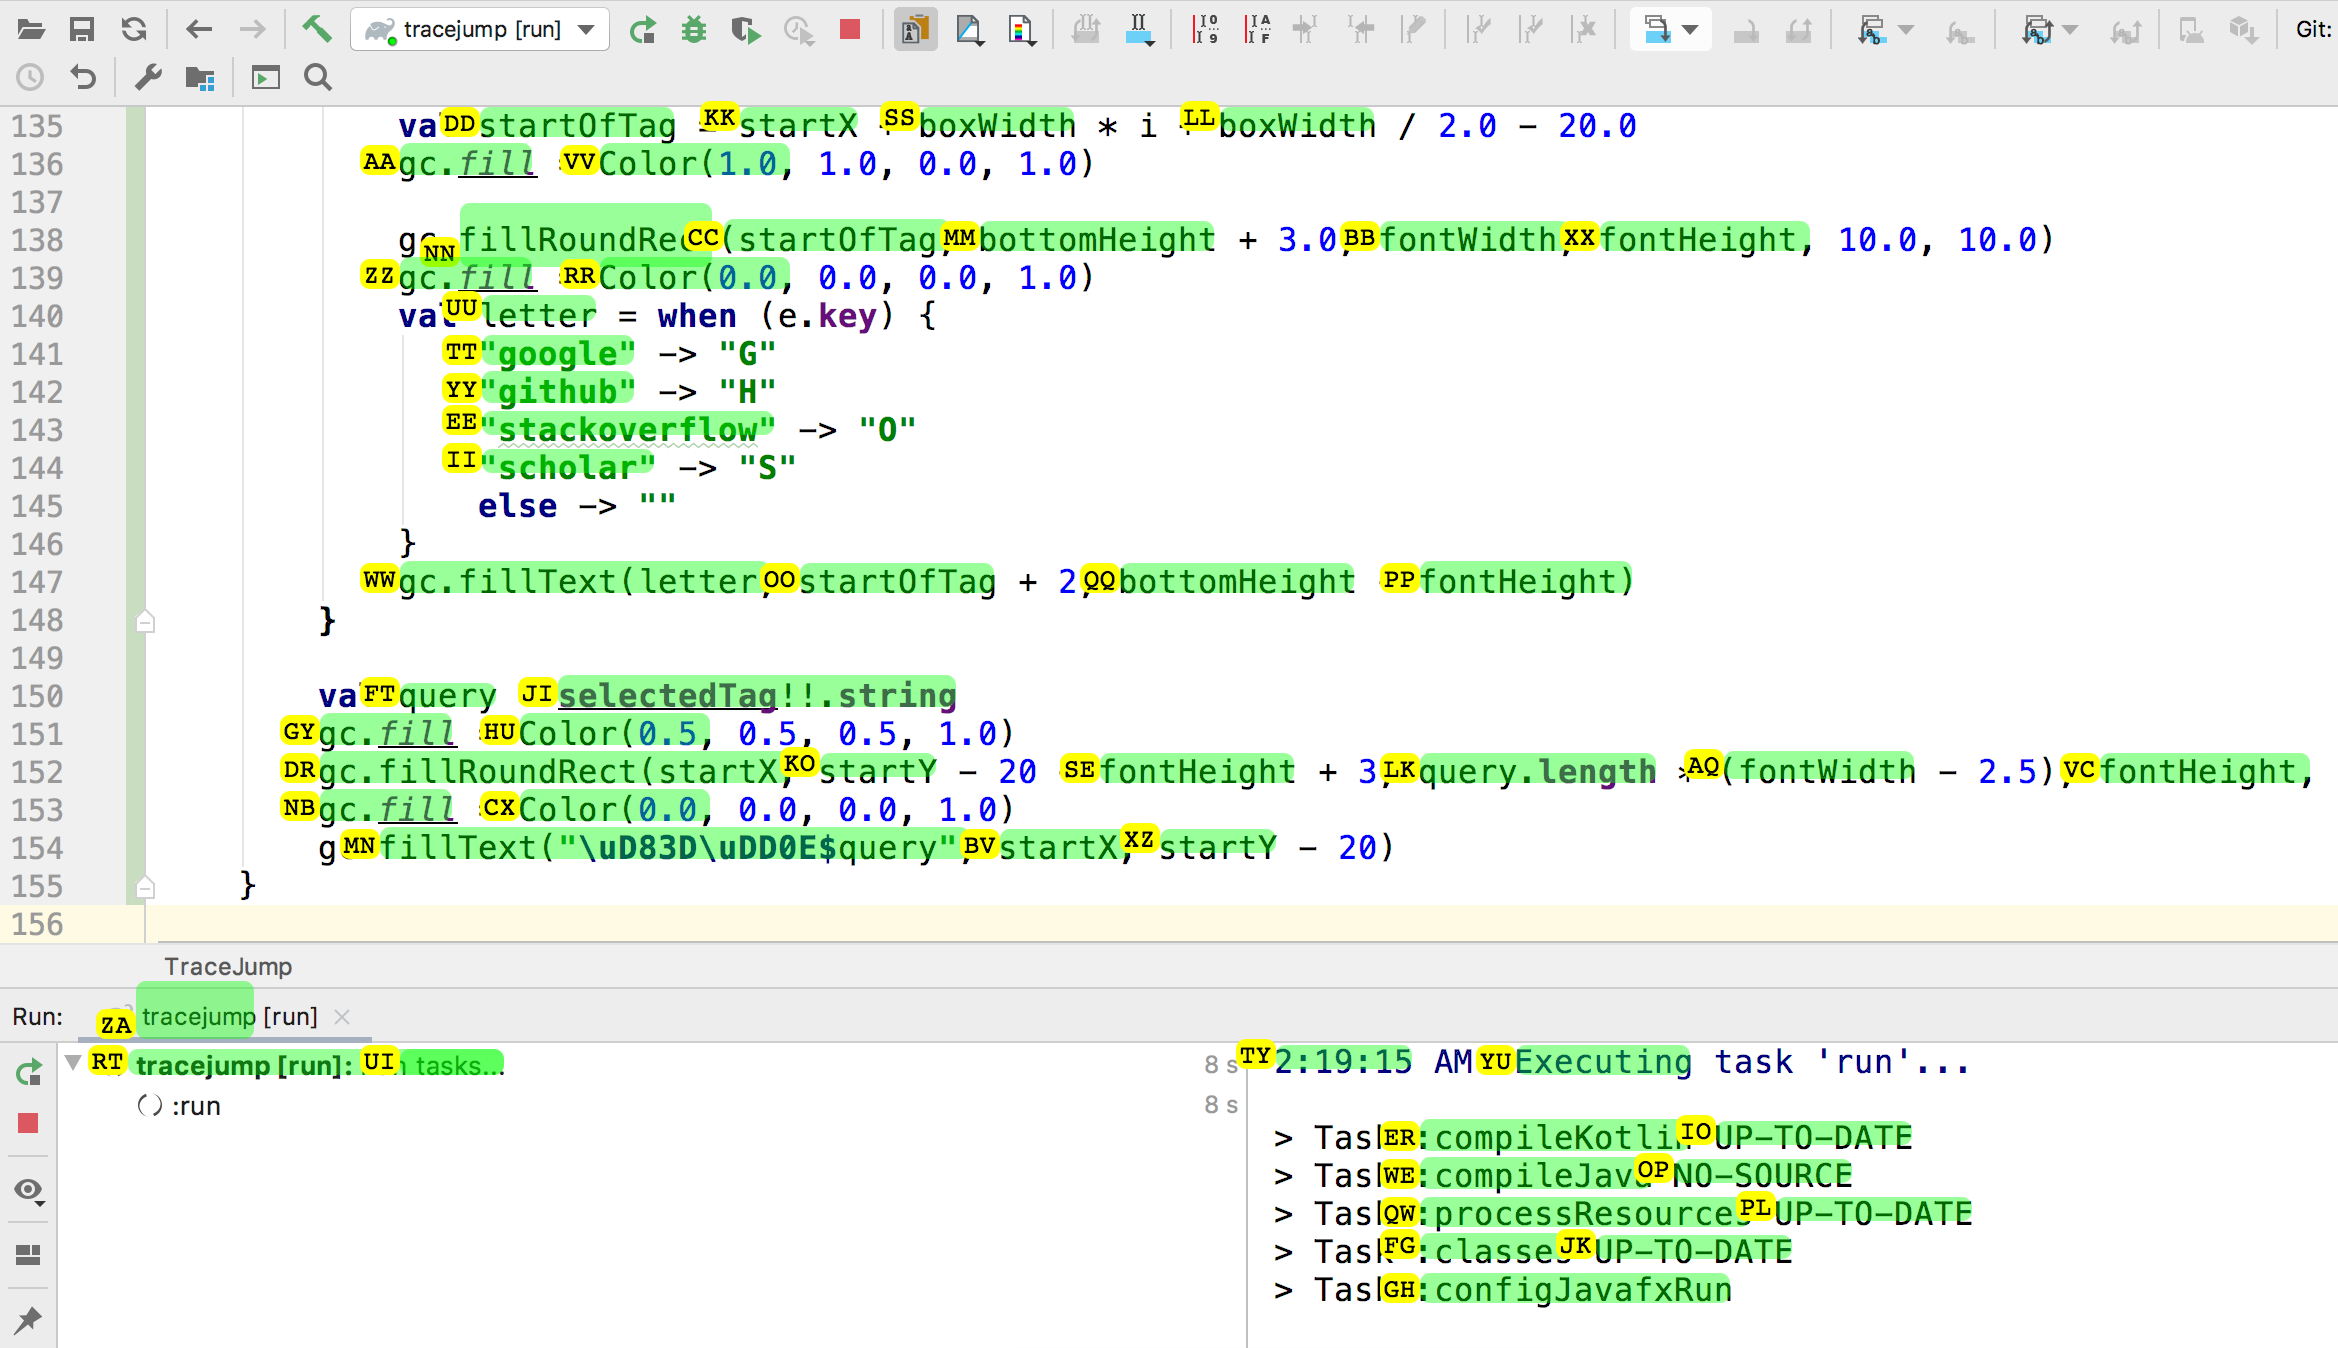
\includegraphics[width=0.4\textwidth,keepaspectratio]{trace_links.png}
    \caption{Trace link annotation with TraceJump.}
    \label{fig:tracejump}
\end{figure}

\section{Discussion}

Our results, while preliminary, indicate a relevance-based ranking over search results can surface some documents that a count-based ranking would omit or obscure, using just a pretrained language model for Simple English with some fine tuning. This is encouraging, as it indicates there is untapped potential for using concordance data to train a language model for contextually relevant document retrieval. However further preprocessing and model architecture improvements are likely necessary in order to achieve competitive results on out-of-vocabulary and out-of-distribution queries.

\subsection{Threats to Validity}\label{subsec:threats}

One threat to validity we have identified is related to the problem of domain mismatch. Our application is primarily intended for inferring the relevance of documentation to a source code snippet, based contextual information in the source and target document. Although our corpus consists of inbound links within documentation sites containing frequent references to API entities, the context may be too dissimilar to be informative in a pure code setting. Ideally, the training set would consist of links exclusively containing code tokens drawn from the same vocabulary. Links within documentation pages may be too broad to infer relevance within other content types based on text alone. We believe it is feasible to refine the dataset by using more selective API extraction techniques as described by~\citet{ma2019easy} and~\citet{ye2016learning, Ye:2018:AAR:3296848.3296902}.

A second threat to validity is the prevalence of autolinking in many knowledge bases and documentation systems. It is common practice in API documentation to use static site generators which are capable of injecting links to named entities in an automatic fashion. We have attempted to mitigate the threat of autolinking by introducing various criteria (cf. Section~\ref{subsec:preprocessing}) to help preserve the intentionality and relevance of a link in its natural context. While PageRank~\cite{page1999pagerank} may have been a stronger baseline in another setting, it assumes documents containing human-generated links, which is not a safe assumption in many software documentation sites.

Partial observability of the TraceJump screen reader is somewhat troublesome, as it can only extract visible text. The application of OCR and screen-reading technology may be less suitable for applications where context is off-screen or distributed unevenly throughout the source document. The OCR tool is prone to misinterpreting certain characters when the font is small or low resolution, and would require further training to be competitive on domain-specific language models. An application-specific integration has the advantage of parsing exact text sequences and would allow the encoder to incorporate context which is not visible on screen. However building application-specific plugins is significantly more time-consuming and less maintainable.

\section{Conclusion}

Searching for documentation is a task that requires devoting some amount of cognitive effort. We present a novel approach to facilitate knowledge discovery by applying language modeling to learn a ranking over concordance-enriched search results from a standard lexical search engine. Our approach works well in the context of lexical search, and can be added to any document retrieval pipeline in a straightforward manner. As a proof of concept, we provide two tools: a visual trace link navigator, capable of annotating links in graphical development environments, and TraceLink, a novel preprocessing architecture for documentation retrieval. Together, these tools cooperate to faciliate knowledge discovery by suggesting relevant documentation to a software development environment. In future work, we hope to evaluate our ranking function on analytics obtained from real users, and introduce a human-in-the-loop reranking functionality.

%%
%% The next two lines define the bibliography style to be used, and
%% the bibliography file.
\bibliographystyle{ACM-Reference-Format}
\bibliography{sample-base}


\end{document}
\endinput
%%
%% End of file `sample-authordraft.tex'.
